\section{Certainty Without Knowing: The Rise of Concentration Inequalities}

\subsection{Bounding the Unseen: Why Concentration Matters}

Where variational inference provides a lens for comparing distributions—quantifying how one belief diverges from another—\textbf{concentration inequalities} do something subtler, and in some ways more radical: they offer guarantees about the behavior of random variables without requiring knowledge of the full distribution at all.

In a philosophical sense, concentration inequalities reflect a kind of probabilistic minimalism. Instead of assuming we know the exact form of \( p(x) \), they ask: \emph{Given only limited information about a random variable—like its mean or its boundedness—how much can we say about its fluctuations?} This is the heart of statistical learning theory: making precise claims about uncertainty in the face of ignorance.

\subsection{A Historical Interlude: From Law of Large Numbers to Hoeffding's Inequality}

The roots of this idea stretch back to the 19\textsuperscript{th} century and the Law of Large Numbers. Early statisticians and physicists were fascinated by the idea that randomness, when repeated, becomes regular. But how fast does this convergence happen? How surprising is a deviation? And can we measure surprise without knowing the full probability distribution?

The modern answers began to crystallize in the mid-20\textsuperscript{th} century, particularly through the work of Wassily Hoeffding. In 1963, he introduced what is now called \textbf{Hoeffding’s inequality}—a result that gives an exponential upper bound on the probability that the sum of bounded independent random variables deviates from its mean. Crucially, it requires no assumptions about the underlying distributions beyond their bounds. This was a revelation: useful certainty, built on minimal assumptions.

Around the same time, inequalities like \textbf{Azuma–Hoeffding} (for martingales) and \textbf{McDiarmid’s inequality} (for bounded differences) emerged to handle more complex dependencies. These tools marked a shift in statistical thinking—from analyzing distributions to bounding deviations.

\begin{tcolorbox}[colback=blue!5!white, colframe=blue!50!black, title=Historical Sidebar: Wassily Hoeffding and Kazuoki Azuma]

    \textbf{Wassily Hoeffding} (1914–1991) was a pioneer of nonparametric statistics and among the first to rigorously study probabilistic inequalities for bounded random variables. His 1963 paper introduced what is now called \emph{Hoeffding’s inequality}, providing exponential bounds without assuming Gaussianity—a crucial breakthrough for learning theory.
    
    \medskip
    
    \textbf{Kazuoki Azuma} contributed a key generalization in the 1960s, extending Hoeffding’s ideas to \emph{martingales}, where variables are dependent but retain a certain fairness property. \emph{Azuma’s inequality} became essential in analyzing online algorithms and sequential decision processes, where independence assumptions no longer hold.
    
    \medskip
    
    Their work laid the foundation for high-probability bounds that are robust, elegant, and distribution-free—ideas that now power modern generalization theory in machine learning.
    
\end{tcolorbox}

\subsection{A Complement to Divergence: KL vs. Concentration}

There is a deep conceptual tension between \textbf{KL divergence} and \textbf{concentration bounds}. KL assumes we know (or approximate) two distributions well enough to compare them. Concentration, on the other hand, assumes almost nothing—and yet still says something.

\begin{itemize}
    \item KL divergence is \emph{global}: it captures average-case discrepancies across the full support of a distribution.
    \item Concentration inequalities are \emph{local}: they bound the likelihood of extreme events, one tail at a time.
\end{itemize}

Together, they represent two sides of the probabilistic coin:
\begin{quote}
\textit{KL divergence tells us how wrong our model is; concentration inequalities tell us how often we’ll be wrong.}
\end{quote}

\begin{figure}[H]
    \centering
    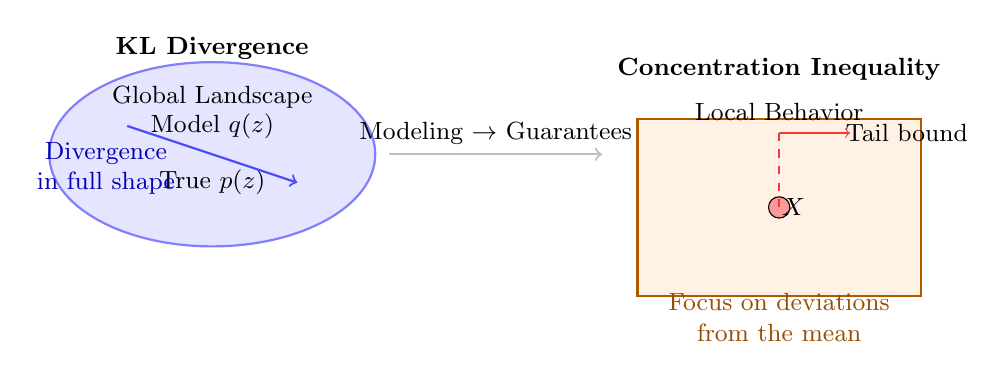
\begin{tikzpicture}[scale=0.9, every node/.style={font=\small}]
    
    % KL Landscape
    \draw[fill=blue!10, draw=blue!50, thick] (-4,1) ellipse (2.3 and 1.3);
    \node at (-4,2.5) {\textbf{KL Divergence}};
    \node at (-4,1.8) {Global Landscape};
    \node at (-4,1.4) {Model \(q(z)\)};
    \node at (-4,0.6) {True \(p(z)\)};
    
    \draw[->, thick, blue!70] (-5.2,1.4) -- (-2.8,0.6);
    \node[align=center, blue!70!black] at (-5.5,0.8) {Divergence\\in full shape};
    
    % Concentration Region
    \draw[fill=orange!10, draw=orange!70!black, thick] (2,-1) rectangle (6,1.5);
    \node at (4,2.2) {\textbf{Concentration Inequality}};
    \node at (4,1.6) {Local Behavior};
    \draw[fill=red!40] (4,0.25) circle (0.15); % Point
    \node at (4.2,0.25) {\(X\)};
    \draw[dashed, thick, red!80] (4,0.25) -- (4,1.3);
    \draw[->, red!80] (4,1.3) -- (5,1.3);
    \node at (5.8,1.3) {Tail bound};
    
    \node[align=center, orange!60!black] at (4,-1.3) {Focus on deviations\\from the mean};
    
    % Arrows between them
    \draw[->, thick, gray!50] (-1.5,1) -- (1.5,1);
    \node at (0,1.3) {Modeling $\rightarrow$ Guarantees};
    
    \end{tikzpicture}
    \caption{KL divergence compares \emph{entire distributions}, like comparing landscapes. Concentration inequalities focus on \emph{specific outcomes}, like predicting rare events. Both are essential perspectives in learning.}
    \label{fig:kl_vs_concentration}
\end{figure}



To further illustrate the philosophical tension between these tools, consider two scientific instruments: the telescope and the microscope. Each reveals a different kind of truth, and each is blind to the other's domain.

\begin{figure}[H]
    \centering
    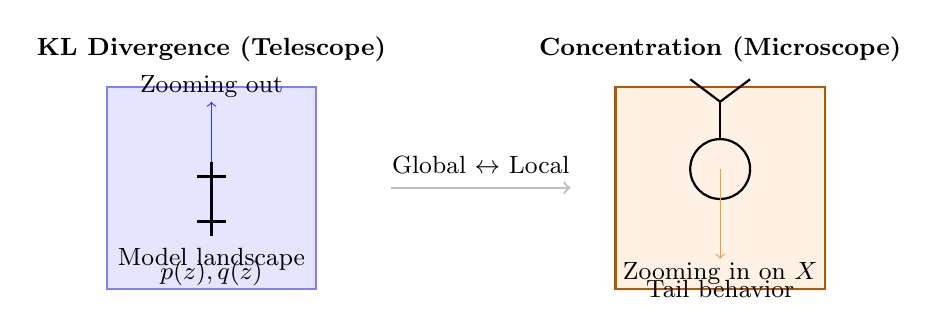
\begin{tikzpicture}[scale=0.95, every node/.style={font=\small}]
    
    % Telescope side
    \draw[fill=blue!10, draw=blue!50, thick] (-5,1.5) rectangle (-2.2,-1.2);
    \node at (-3.6,2) {\textbf{KL Divergence (Telescope)}};
    \draw[thick] (-3.6,0.5) -- (-3.6,-0.5);
    \draw[thick] (-3.8,0.3) -- (-3.4,0.3);
    \draw[thick] (-3.8,-0.3) -- (-3.4,-0.3);
    \node at (-3.6,-0.8) {Model landscape};
    \node at (-3.6,-1.0) {\(p(z), q(z)\)};
    \draw[->, blue!80] (-3.6,0.5) -- (-3.6,1.3);
    \node at (-3.6,1.5) {Zooming out};
    
    % Microscope side
    \draw[fill=orange!10, draw=orange!70!black, thick] (1.8,1.5) rectangle (4.6,-1.2);
    \node at (3.2,2) {\textbf{Concentration (Microscope)}};
    
    \draw[thick] (3.2,0.4) circle (0.4); % microscope lens
    \draw[thick] (3.2,0.8) -- (3.2,1.3); % body
    \draw[thick] (3.2,1.3) -- (2.8,1.6);
    \draw[thick] (3.2,1.3) -- (3.6,1.6);
    \draw[->, orange!80] (3.2,0.4) -- (3.2,-0.8);
    \node at (3.2,-1.0) {Zooming in on \(X\)};
    \node at (3.2,-1.2) {Tail behavior};
    
    % Arrow between them
    \draw[->, thick, gray!50] (-1.2,0.15) -- (1.2,0.15);
    \node at (0,0.45) {Global $\leftrightarrow$ Local};
    
    \end{tikzpicture}
    \caption{KL divergence acts like a telescope: comparing global shapes of distributions. Concentration inequalities act like a microscope: analyzing local behavior around expected values.}
    \label{fig:telescope_vs_microscope}
\end{figure}



This distinction is crucial in machine learning. While KL divergence informs model selection and training objectives (like the ELBO), concentration inequalities inform generalization: how well does a model trained on finite data perform on unseen examples? One is about belief. The other, about behavior.

\subsection{The Philosophical Tension: Certainty From Ignorance}

The philosophical beauty of concentration inequalities lies in their epistemic modesty. They do not pretend to model the world precisely. Instead, they offer \emph{robust} guarantees—bounds that hold regardless of the details. This robustness is why concentration inequalities became foundational in learning theory: they allow us to reason about uncertainty with minimal assumptions.

They are the mathematics of restraint. While variational inference asks, ``How do I best approximate what I don’t know?'', concentration bounds ask, ``What can I safely assume, even when I know very little?''

\begin{tcolorbox}[colback=gray!5!white, colframe=black!75!white, title={Historical Sidebar: Carnap and the Collapse-Proof Dream of Inductive Logic}]

    \textbf{Rudolf Carnap} (1891–1970) was one of the intellectual architects of \textbf{logical positivism}, a movement born in the Vienna Circle that sought to reconstruct philosophy on the secure foundation of logic and empirical verification. 
    
    For a time, it seemed almost plausible: that all knowledge could be derived from formal logic and observation, and that ambiguity, metaphysics, and speculation could be eliminated like bad code.
    
    Then came \textbf{Gödel}.
    
    His incompleteness theorems (1931) blew a hole in the dream. No formal system could prove all the truths about arithmetic. Worse: any sufficiently powerful system would contain true statements it could never prove. The very idea of a self-contained, self-verifying logic was dead on arrival.
    
    Carnap didn’t abandon the project—he \textit{revised} it.
    
    \medskip
    
    Where others saw Gödel’s results as a fatal wound, Carnap saw an opportunity: a reason to pivot from \textbf{deductive certainty} to \textbf{inductive plausibility}. If knowledge couldn’t be built from axioms alone, maybe it could be shaped by rational degrees of belief.
    
    In works like \textit{The Logical Foundations of Probability} (1950), Carnap launched a new program: the formalization of \textbf{inductive logic}. He attempted to assign logical probabilities to hypotheses based on their structure, aiming for:
    
    \begin{itemize}
        \item Objective prior probabilities,
        \item Rule-based belief updating,
        \item A logic of confirmation grounded in syntax.
    \end{itemize}
    
    \medskip
    
    But even this revised project struggled. Carnap's system couldn’t escape a fatal ambiguity: there’s no unique, rational way to assign priors. Attempts to axiomatize induction ran into paradoxes of symmetry, arbitrariness, and philosophical disagreement.
    
    Still, Carnap’s work seeded modern fields like:
    
    \begin{itemize}
        \item \textbf{Bayesian inference}, where priors are subjective but updated by rules;
        \item \textbf{Variational inference}, where logic is replaced by optimization;
        \item \textbf{Information theory}, where beliefs are compressed and quantified.
    \end{itemize}
    
    \medskip
    
    \textbf{Carnap’s wager was that even after Gödel, rational belief could be formalized.}  
    Not as certainty—but as structured uncertainty.
    
    He didn’t solve the problem of induction.  
    But he showed it could be mathematized—at least enough to build something useful on top of it.
    
\end{tcolorbox}
        

\subsection{Prelude to Learning Theory}

As machine learning grew from statistical roots into an algorithmic science, this duality became central. Variational methods power deep generative models and structured approximations. Concentration inequalities underpin PAC learning, uniform convergence, and generalization guarantees.

In the sections that follow, we’ll see how these philosophical tools—KL divergence and concentration inequalities—come together in modern learning systems. One provides a language for inference. The other, for confidence.

\begin{quote}
\textit{To learn is to balance belief and behavior: what we think is true, and how often we’ll be wrong.}
\end{quote}










